\section{Setup} 
\subsection{Requirements}
In this section all of the requirements are described.
\subsubsection{Operating system}
\textit{Soldino}'s development environment is available for the following operating systems:
\begin{itemize}
	\item\textbf{Ubuntu 18.04.2 LTS} or later;
	\item\textbf{Windows 10} all versions.
\end{itemize}
In the manual all instructions are provided in order to configure and run \textit{Soldino} on both operating system.
\subsubsection{Hardware}
 
\begin{itemize}
	\item  \textbf{Processor}: Pentium 4 (dual core) or newer;
	\item \textbf{RAM}: 2GB or more;
	\item \textbf{Hard drive}: 1GB of hard drive space;
	\item \textbf{Internet connection}: required for run Soldino DApp;
\end{itemize}

\subsubsection{Browser}
\textit{Soldino} is accessible through a web interface. The currently most 
recent versions of the following browsers are supported:
\begin{itemize}
	\item \textbf{Mozilla Firefox}: version 64 or newer;
	\item \textbf{Google Chrome}: version 71 or newer.
\end{itemize}

\subsubsection{Tools}
The following tools are needed:
\begin{itemize}
	\item \textbf{Git}: a famous control version system: \textit{Soldino}'s 
	repository\glosp is hosted on GitHub\glo;
	\item \textbf{Node.js\glo}: a framework needed for installing dependencies;
	\item \textbf{Npm\glo}: a packets manager for JavaScript language, used by default by node.js;
	\item \textbf{Truffle\glo}: needed to write and deploy contracts with ease;
	\item \textbf{Ganache\glo}: needed to put up a local Ethereum network and check 
	transactions in it. You can choose between Ganache GUI(UI) and ganache-cli(command-line) or have both;
	\item \textbf{Metamask\glo}: a browser plugin\glosp used as a virtual wallet;
	\item \textbf{Surge.sh\glo}: a web platform chosen for hosting the website 
	interface of Soldino.
\end{itemize}

\subsubsection{Dependencies}
\textit{Soldino} depends on many packages. All these dependencies can be found 
in the file \texttt{package.json} which is in the root folder of the project.\\
The packages required to execute the software \textit{Soldino} are listed below.\\

\renewcommand{\arraystretch}{1.5}
\rowcolors{2}{pari}{dispari}
\begin{longtable}{ 
		>{\centering}p{0.4\textwidth} 
		>{\centering}p{0.4\textwidth}
	}
	\caption{Packages required for software usage}\\
	\rowcolorhead
	\textbf{\color{white}Software} & 
	\textbf{\color{white}Version}
	\tabularnewline  
	\endhead	
	
	% voci prese da package.json, repo "Soldino-PoC, ramo "develop"


	react-text-mask & $\geq$5.4.4
	\tabularnewline
	commondir &$\geq$1.0.1
	\tabularnewline
	history &$\geq$4.7.2
	\tabularnewline
	prop-types &$\geq$15.7.2\tabularnewline
	react &$\geq$16.8.3\tabularnewline
	react-dom &$\geq$16.8.3\tabularnewline
	react-number-format &$\geq$4.0.6\tabularnewline
	react-redux &$\geq$6.0.1\tabularnewline
	react-router &$\geq$4.3.1\tabularnewline
	react-router-dom &$\geq$4.3.1\tabularnewline
	react-router-redux &$\geq$4.0.8\tabularnewline
	react-scripts &$\geq$2.1.8\tabularnewline
	redux &$\geq$4.0.1\tabularnewline
	redux-thunk &$\geq$2.3.0\tabularnewline
	web3 & 1.0.0-beta.37\tabularnewline
	
\end{longtable}

Other packages, listed below, are required for the development.
\renewcommand{\arraystretch}{1.5}
\rowcolors{2}{dispari}{pari}
\begin{longtable}{ 
		>{\centering}p{0.4\textwidth} 
		>{\centering}p{0.4\textwidth}
	}
	\caption{Packages required for development}\\
	\rowcolorhead
	\textbf{\color{white}Software} & 
	\textbf{\color{white}Version}
	\tabularnewline  
	\endhead	
	
	% voci prese da package.json, repo "Soldino-PoC, ramo "develop"
	eslint & 5.12.0\tabularnewline
	eslint-config-airbnb &$\geq$17.1.0\tabularnewline
	eslint-loader & $\geq$2.1.2\tabularnewline
	eslint-plugin-import & $\geq$2.16.0\tabularnewline
	eslint-plugin-jsx-a11y & $\geq$6.2.1\tabularnewline
	pre-commit & $\geq$1.2.2\tabularnewline
	truffle-contract & $\geq$4.0.6\tabularnewline
	ganache-cli & $\geq$6.4.3
\end{longtable}
\pagebreak
\subsection{Installing}
\textit{Soldino} can be installed on multiple Operating System but we recommend to use a 
Unix environment because some functionalities do not work on Windows, for example solidity-coverage.\\
To start \textit{Soldino} follow these instructions to avoid errors during the installation. Instructions are grouped by technology. Each of those can contain references to a particular OS. Where the steps are the same we have not indicate nothing; otherwise we divided the steps in different paragraphs.
\subsubsection{Browser}
You can get the latest Google Chrome version 
\href{https://www.google.com/chrome/}{here} or the latest Firefox version \href{https://www.mozilla.org/en-US/firefox/new/}{here}
\subsubsection{Git}
\paragraph{Linux} \mbox{} \\ \mbox{} \\
You have to type this script in the shell to install Git: 
\texttt{sudo apt install git}.
\paragraph{Windows} \mbox{} \\ \mbox{} \\
Download Git from: \url{https://git-scm.com/download/win}. \\
Choose "Save file" and at the end of download go to destination directory, launch executable file and follow the instructions until the end.

\subsubsection{Node.js and npm}
\paragraph{Linux} \mbox{} \\ \mbox{} \\
To install the latest Node.js version copy in the terminal the following commands:
\begin{enumerate}
	\item \texttt{curl -sL https://deb.nodesource.com/setup\_11.x | sudo -E bash -}
	\item \texttt{sudo apt install -y nodejs}
\end{enumerate} 
You can check if \texttt{node} was installed correctly by typing in the 
terminal: \texttt{node -v}.\\ \\
\textbf{Note}: that npm\glosp is installed with the previous commands. You can check if \texttt{npm} was installed correctly by typing in the 
terminal: \texttt{npm -v}.\\
\paragraph{Windows} \mbox{} \\ \mbox{} \\
To install the last Node.js\glosp version go to the following link: \url{https://nodejs.org/it/} and take recommended version.
Choose "Save file" and at the end of download go to destination directory, launch \texttt{.msi} file and follow the instructions until the end.
For \textbf{npm} run these on eleveted command prompt (admin):
\begin{itemize}
	\item \texttt{npm install npm@latest -g};
	\item \texttt{npm install ---global ---production windows-build-tools}.
\end{itemize}

\subsubsection{Truffle}
You should check you have the truffle requirements:
\begin{itemize}
	\item an OS among Linux, Windows and MacOS (prefer Linux);
	\item NodeJS v10.15.1 or later (we picked version 11);
	\item Node Package Manager (npm\glo).
\end{itemize}
then you can install Truffle by running the command: \texttt{npm install -g truffle}

%Non credo Ganche serva nella versione finale

\subsubsection{Ganache}
\paragraph{Linux - Ganache GUI} \mbox{} \\ \mbox{} \\
Ganache is a part of Truffle suite and is used to put up a local blockchain.
There are three steps to install Ganache GUI:
\begin{enumerate}
	\item you can download the Ganache executable at this link \url{https://truffleframework.com/ganache}, clicking on the download button;
	\item now you have to give the permissions to make the Ganache file executable. Go to download destination directory and open new terminal. Then run this command: \\\texttt{chmod +x path-of-the-appimage/name-of-downloaded-file.AppImage};
	\item double click on executable file and follow the instructions until the end.
\end{enumerate}
\paragraph{Linux - ganache-cli} \mbox{} \\ \mbox{} \\
Ganache-cli is the same things as previous one, but you can use Ganache only by command line.
To install ganache-cli, open a terminal and run: \\ \texttt{sudo npm install -g ganache-cli} .
\paragraph{Windows - Ganache GUI} \mbox{} \\ \mbox{} \\
On Windows download from here: \\
\url{https://truffleframework.com/ganache}. \\
Then, double click on executable file and follow instructions until the end.
\paragraph{Windows - ganache-cli} \mbox{} \\ \mbox{} \\ 
For \textbf{ganache-cli} run these on eleveted command prompt (admin):\\
\texttt{npm install -g ganache-cli} .
\subsubsection{MetaMask}
You can add it to your browser in this way:
\begin{itemize}
	\item Chrome:  \href{https://chrome.google.com/webstore/search/metamask?hl=it}{https://chrome.google.com/webstore/search/metamask?hl=it};
	\item Firefox: \href{https://addons.mozilla.org/it/firefox/addon/ether-metamask/?src=search}{https://addons.mozilla.org/it/firefox/addon/ether-metamask/?src=search}.
\end{itemize}


\subsubsection{Surge}
You have to install Surge\glosp by executing the shell command: \texttt{npm install -g surge}.


\subsection{Configuration}
This section shows how to configure your work environment, so that it's the same as ours, in order to minimize the number and entity of troubles you will occur in.\\
Make sure to configure the tools in order. In particular, Truffle requires that Ganache is opened and is configured to execute successfully.
% clona la repo; apri truffle, apri ganache, apri browser con metamask, setta
\subsubsection{Cloning the repository}
You have to clone the \textit{Soldino} repository on GitHub: open the command line, move to the directory where you want place Soldino, then use \texttt{git clone https://github.com/8LabSolutions/Soldino-PoC}. After that use command: \texttt{cd Soldino-PoC} to move into directory.
% and then use \texttt{git checkout final}.  

\subsubsection{Ganache GUI}
You have to go to the folder where you've put Ganache, and open it with double click.
\begin{figure}
	\centering
	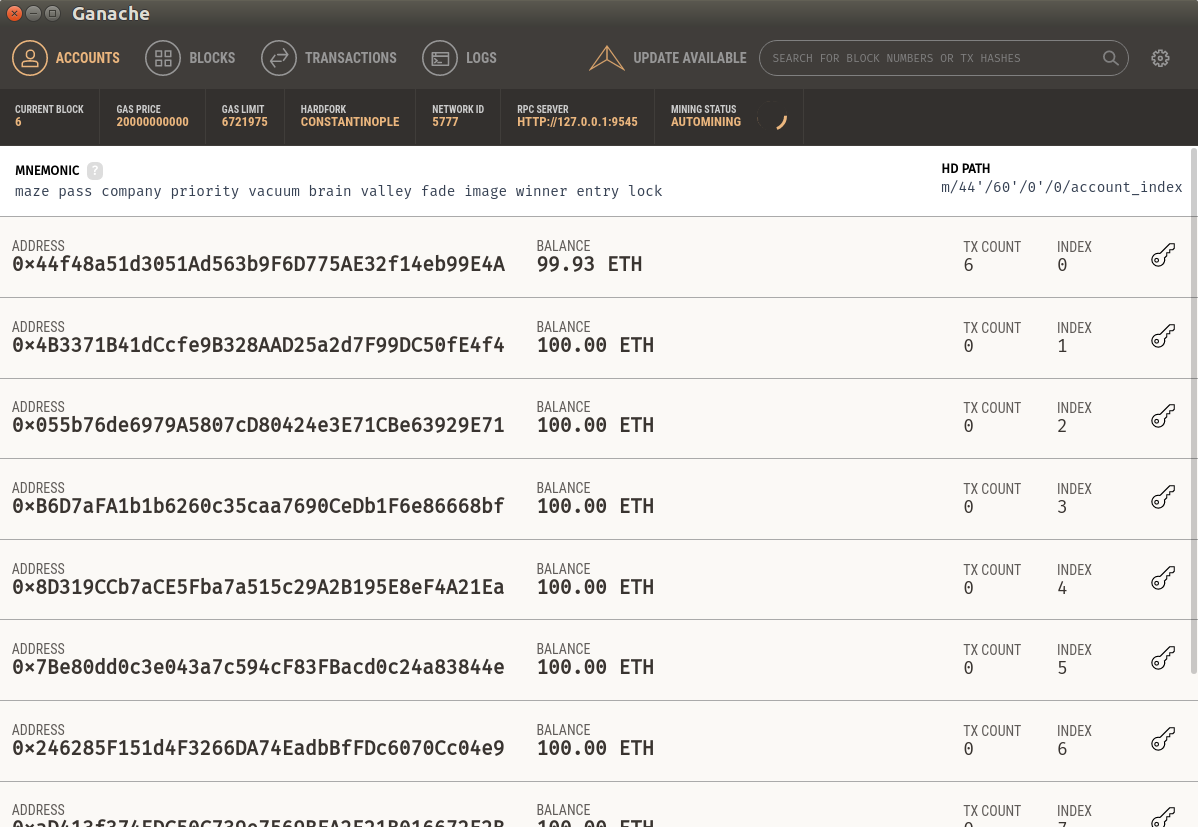
\includegraphics[scale=0.25]{res/images/ganache-ui.png}
	\caption{Ganache GUI: from top to bottom you can see the menu bar, the current configuration, the mnemonic, and the interface of the selected menu option}
\end{figure}
Then you have to click on the cogwheel at the top left corner to access Ganache settings and make sure you've matched the following settings (most of which are defined in \texttt{truffle-config.js}) on each respective window:
\begin{itemize}
	\item Server:
	\begin{itemize}
		\item hostname: \texttt{127.0.0.1};
		\item port number: \texttt{9545};
		\item network id: any (you can keep the default one).
	\end{itemize}
	\item Account \& keys\glo:
	\begin{itemize}
		\item nothing to configure here, but you should have a look at the \textbf{mnemonic}: it will help you later.
	\end{itemize}
\end{itemize}

\subsubsection{Ganache-cli}
If you use \textbf{ganache-cli} open terminal on your project directory and run this command: \\
\texttt{ganache-cli -p \#portnumber} (9545 recommended)\\
Keep open this terminal during use \textit{Soldino} and use for other steps another command line.
You can exit by typing \texttt{ctrl + C}.

\subsubsection{Truffle}
The configuration of Truffle is defined in the file \texttt{truffle-config.js} in the root directory of \textit{Soldino}.
On your command line type the following commands:
\begin{itemize}
	\item \texttt{truffle console}\\
	opens the truffle environment in the shell under the configuration defined in truffle-config.js. From now on, every command is executed in the truffle environment, from which you can exit double typing \texttt{ctrl + C}.
	\item \texttt{compile}\\
	to compile the contracts: these are compiled in in a .json\glosp format (which enables interaction with the frontend) and put into the folder defined in \texttt{truffle-config.js} at \texttt{contracts\_build\_directory} (in our case the location is \texttt{./src/contracts\_build})
	\item \texttt{migrate -{}-network development}\\
	puts the contracts runnning on the blockchain\glo. 
\end{itemize}

\subsubsection{MetaMask}
It's necessary to create an account.
\begin{itemize}
	\item open MetaMask on your browser
	\item select get started
	\item select import wallet
	\item use the seed phrase (MNEMONIC), copy and paste it from ganache(GUI) or terminal(ganache-cli) to metamask's textbox, then put your password and confirm.
\end{itemize}
Now your account is up and synchronized with Ganache.
Now you have to connect the wallet to Ganache network. Ganache settings are exposed in the Ganache GUI just above the mnemonic.
Let's synchronize MetaMask to the same network. On the top right corner there is a drop-down menu to select the network. Select \texttt{Custom RPC} to set your own local network.\\
You are now in the MetaMask advanced settings screen. In the field \texttt{Net Network} click on \texttt{Show Advanced Options} to open the form, then insert these data:
\begin{enumerate}
	\item \textbf{New RPC URL}: http://127.0.0.1:9545 (the port number matches the one in truffle-config.js);
	\item \textbf{Nickname}: the name you wanna give to your network;
	\item \textbf{save} when you're done.
\end{enumerate}
MetaMask is now connected to Ganache.\\

\noindent To enable transactions on your local test network, you can find free ether\glosp for testing networks on this site: \href{https://faucet.metamask.io/}{https://faucet.metamask.io/}.

\subsubsection{Npm}
\paragraph{Linux} \mbox{} \\ \mbox{} \\
Open terminal on \textit{Soldino} project directory and run:
\texttt{sudo apt-get install build-essential} \\
It's time to install all dependencies by running: \texttt{npm install}
\paragraph{Windows} \mbox{} \\ \mbox{} \\
Install all dependecies in the same way of Linux: open terminal on \textit{Soldino} project directory and run: \texttt{npm install}.
% PUT CUBIT TO METAMASK

\subsection{Running}
Now that you have all the required software installed and configured, it's time to get it up running.\\
All you have to do is moving to the root directory of Soldino and prompt
\begin{itemize}
	\item[]\texttt{npm start}
\end{itemize}
This will open the website on your default browser at the address \texttt{http://127.0.0.1:3000} and allow you to explore it.
\subsection{Deploy on Ropsten Infura}


%\subsection{Deploying}
%This part shows you how to deploy contracts with Truffle and have them up running on Soldino.
%
% qua c'è surge, il deploy su ropsten, etc. VAnno cambiati alcuni file nei parametri di configurazione
% 